%%%%%%%%%%%%%%%%%%%%%%%%%%%%%%%%%%%%%%%%%
% Memo
% LaTeX Template
% Version 1.0 (30/12/13)
%
% This template has been downloaded from:
% http://www.LaTeXTemplates.com
%
% Original author:
% Rob Oakes (http://www.oak-tree.us) with modifications by:
% Vel (vel@latextemplates.com)
%
% License:
% CC BY-NC-SA 3.0 (http://creativecommons.org/licenses/by-nc-sa/3.0/)
%
%%%%%%%%%%%%%%%%%%%%%%%%%%%%%%%%%%%%%%%%%

\documentclass[letterpaper,11pt]{texMemo} % Set the paper size (letterpaper, a4paper, etc) and font size (10pt, 11pt or 12pt)

\usepackage{parskip} % Adds spacing between paragraphs
\usepackage[colorlinks]{hyperref}
\usepackage{graphicx}
\usepackage{gensymb}
\usepackage{float}
\usepackage{listings}
\usepackage{csvsimple}
\hypersetup{citecolor=DeepPink4}
\hypersetup{linkcolor=red}
\hypersetup{urlcolor=blue}
\usepackage{cleveref}
\setlength{\parindent}{15pt} % Indent paragraphs

%----------------------------------------------------------------------------------------
%	MEMO INFORMATION
%----------------------------------------------------------------------------------------

%----------------------------------------------------------------------------------------
%	MEMO INFORMATION
%----------------------------------------------------------------------------------------

\memoto{Dr.Jeff McGough} % Recipient(s)

\memofrom{Benjamin Lebrun} % Sender(s)

\memosubject{Homework 3} % Memo subject

\memodate{\today} % Date, set to \today for automatically printing todays date

%\logo{\includegraphics[width=0.1\textwidth]{logo.png}} % Institution logo at the top right of the memo, comment out this line for no logo

%----------------------------------------------------------------------------------------

\begin{document}


\maketitle % Print the memo header information

%----------------------------------------------------------------------------------------
%	MEMO CONTENT
%----------------------------------------------------------------------------------------

\section*{Problem 8.1}
\subsection*{Problem statement}
Assume that you are working in a large event center which has beacons located around the 
facility. Estimate the location of a robot, $(a,b,c)$, if the $(x,y,z)$ location of the beacon 
and the distance from the beacon to the robot, $d$, are given in the table below.

\csvautotabular{../P1.csv}

% \begin{tiny}
%     \begin{lstlisting}
%     import pylab as plt
%     plt.plot(x,y,'b.')
%     plt.show()
%     \end{lstlisting}
% \end{tiny}

\subsection*{Solution approach and algorithm description.}


\[
    2(a_j-a_i)x + 2(b_j-b_i)y  = r_i^2 - r_j^2 - a_i^2 + a_j^2 - b_i^2 + b_j^2
\]

\[
    2(a_k-a_i)x + 2(b_k-b_i)y = r_i^2 - r_k^2  - a_i^2 + a_k^2 - b_i^2  + b_k^2  .
\]

%
%\begin{figure}[ht]
%\caption{Graphed path of Robot}
%\centering
%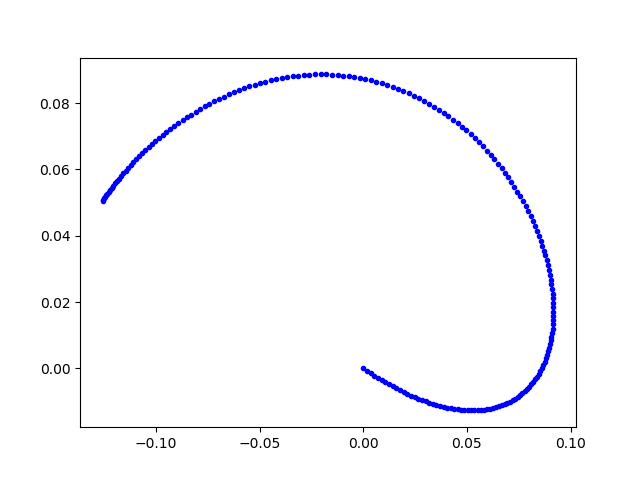
\includegraphics[scale=0.45]{img/P4a.png}
%\end{figure}

\newpage
\subsection*{Code for Problem 5}
\begin{tiny}
\lstinputlisting{../P1.m}
\end{tiny}

\subsection*{Matlab output}
\begin{tiny}
\lstinputlisting{../solutionFile.txt}
\end{tiny}

\newpage
\section*{Problem 8.2}
\subsection*{Problem statement}
If you are using a laser diode to build a distance sensor, you need some method to determine the
travel time. Instead of using pulses and a clock, try using phase shifts. What is the wavelength 
of the modulated frequency of 10MHz? If you measure a 10 degree phase shift, this value corresponds 
to what distances? What if the phase shift measurement has noise: zero mean with standard deviation 
0.1? How does one get a good estimate of position if the ranges to be measured are from 20 meters 
to 250 meters?

\subsection*{Solution approach and algorithm description.}

To find our wavelength we use the following equation

\[
    \lambda = \frac{c}{v}
\]

Where $c$ is the speed of light, $\lambda$ is our wavelength, and $v$ is our frequency. Thus

\[
    \lambda = \frac{3*10^8 \frac{m}{s}}{10*10^6}
\]

We find that $\lambda = 30$ meters.

For a $10\degree$ phase shift, we use the equation for phase shift of the wavelength distance

\[
    D = \frac{\lambda}{4\pi} \theta
\]

$D = \frac{10}{360}30 = 0.8333$ meters.

For the full trip this would be $0.8333 + 30n$ for $n = 0,1,2,3\dots$
for some values of $n$, would then create the solutions $=0.8333, 30.8333, 60.8333,\dots$

For a phase shift measurement with noise, we pick a second frequency that isn't a factor of 
10 in the MHz range, then use the same calculations with a measured phase shift to find a second
set of points and correlate the answer from the point that the two share with our standard deviation 
factored into the calculation, in this case with any distance between the 20 and 250 meters 
range.


\newpage
\section*{Problem 9.1}
\subsection*{Problem statement}
Assume you have a laser triangulation system as shown in Fig. 9.2 given by (9.1) and that $f  = 8$mm,
$b=30$cm. What are the ranges for $\alpha$ and $u$ if we need to measure target distances in a region
(in cm) $20 < z < 100$ and $10<x<30$?

\subsection*{Solution approach and algorithm description.}

For the given range of $x$ and $z$, we know that the angle $\alpha$ can only reasonably be in the range
$0<\alpha<90\degree$, given this, we find the maximum and minimum for these angles with the equations

\[
    x = \frac{b u}{f\cot \alpha + u},  \quad
z = \frac{b f}{f\cot \alpha + u}
\]

with our given vales, these become

\[
    x = \frac{30 u}{0.8\cot \alpha + u},  \quad
z = \frac{30 * 0.8}{0.8\cot \alpha + u}
\]

With a calculator defining the limits to be $0<\alpha<90\degree$, $20 < z < 100$ and $10<x<30$. Our answers become 
$45\degree<\alpha<71.565\degree$ and $1.6\cot \alpha < u < -0.8(\cot \alpha - 3)$. For our range of $u$ we use the
maximum and minimum found for $\alpha$, which then defines $u$ along the range $0.53<u<2.1334$ cm.

\newpage
\section*{Problem 9.1}
\subsection*{Problem statement}
ssume you have two cameras that are calibrated into a stereo pair with a baseline of 10cm, and focal depth of 7mm. If the error is 10\% 
on $v_1$ and $v_2$, $v_1=2$mm and $v_2=3mm$, what is the error on the depth measurement $z$? Your answer shoudl be a percentage relative 
to the error free number. Hint: If $v_1=2$ then a 10\% error ranges from 1.8 to 2.2 [Although not required, another way to approach this problem is the total differential from calculus.]

\subsection*{Solution approach and algorithm description.}


\end{document}